\documentclass[a4paper, 14pt]{extarticle}

% Поддержка языков
\usepackage[english, russian]{babel} 

% Настройка кодировок
\usepackage[T2A]{fontenc}
\usepackage[utf8]{inputenc}

% Настройка шрифтов
\usepackage{fontspec}
\setmainfont[Ligatures=TeX]{Times New Roman} % Шрифт для основного текста документа
\setsansfont[Ligatures=TeX]{Arial}
\setmonofont{Consolas} % Шрифт для кода

\usepackage{tocloft}

% Настройка отступов от краев страницы
\usepackage[left=3cm, right=1.5cm, top=2cm, bottom=2cm]{geometry}

\usepackage{titleps} % Колонтитулы
\usepackage{subfig} % Для подписей к рисункам и таблицам
\usepackage{graphicx} % для вставки картинок
\graphicspath{{./img/}} % Путь до папки с изображениями
% Пакет для отрисовки графиков
\usepackage{tikz}
\usetikzlibrary{arrows,positioning,shadows}
\usepackage{stmaryrd} % Стрелки в формулах
\usepackage{indentfirst} % Красная строка после заголовка
\usepackage{hhline} % Улучшенные горизонтальные линии в таблицах
\usepackage{multirow} % Ячейки в несколько строчек в таблицах
\usepackage{longtable} % Многостраничные таблицы
\usepackage{paralist,array} % Список внутри таблицы
\usepackage[normalem]{ulem}  % Зачеркнутый текст
\usepackage{upgreek, tipa} % Красивые греческие буквы
\usepackage{amsmath, amsfonts, amssymb, amsthm, mathtools} % ams пакеты для математики, табуляции
\usepackage{nicematrix} % Особые матрицы pNiceArray

\linespread{1.5} % Межстрочный интервал
\setlength{\parindent}{1.25cm} % Табуляция
\setlength{\parskip}{0cm}

% Пакет для красивого выделения кода
\usepackage{minted}
\setminted{fontsize=\footnotesize}

% Настройка оглавления
\renewcommand{\contentsname}{Содержание}
\renewcommand{\cftsecleader}{\cftdotfill{\cftdotsep}} % точки между главой и номером
% Добавляем гипертекстовое оглавление в PDF
\usepackage[
bookmarks=true, colorlinks=true, unicode=true,
urlcolor=black,linkcolor=black, anchorcolor=black,
citecolor=black, menucolor=black, filecolor=black,
]{hyperref}

% Убрать переносы слов
\tolerance=1
\emergencystretch=\maxdimen
\hyphenpenalty=10000
\hbadness=10000

\newpagestyle{main}{
	% Верхний колонтитул
	\setheadrule{0cm} % Размер линии отделяющей колонтитул от страницы
	\sethead{}{}{} % Содержание {слева}{по центру}{справа}
	% Нижний колонтитул
	\setfootrule{0cm} % Размер линии отделяющей колонтитул от страницы
	\setfoot{}{\thepage}{} % Содержание {слева}{по центру}{справа}
}
\pagestyle{main}
\pagenumbering{arabic}

% НОВЫЕ КОМАНДЫ
\newcommand{\deriv}[2]{\frac{\partial #1}{\partial #2}}
\newcommand{\n}{\par}
\newcommand{\percent}{\mathbin{\%}}

% Заменяем Рис. на Рисунок
\addto\captionsrussian{\renewcommand{\figurename}{Рисунок}}

% Изменение формата подписей
% Стиль номера таблицы/рисунка #1-Таблица/Рис. #2-номер
\DeclareCaptionLabelFormat{custom}
{%
	#1 #2
}
% Стиль разделителя номера таблици/рисунка и названия таблицы/рисунка
\DeclareCaptionLabelSeparator{custom}{$-$}
% Стиль формата #1-номер таблицы/рисунка #2-разделитель #3-название
\DeclareCaptionFormat{custom}
{%
	#1 #2 #3
}

\captionsetup
{
	format=custom,%
	labelsep=custom,
	labelformat=custom
}

% ПЕРЕГРУЗКА УЖЕ СУЩЕСТВУЮЩИХ КОМАНД
\renewcommand{\epsilon}{\varepsilon} % Заменить знак эпсилон
\renewcommand{\phi}{\varphi}
\renewcommand{\kappa}{\varkappa}
\renewcommand{\lambda}{\uplambda}


\begin{document}
	\newcommand{\Faculty}{Факультет программной инженерии и компьютерной техники}

\newcommand{\TeacherPosition}{}
\newcommand{\TeacherName}{Белокон Юлия Алексеевна}

\newcommand{\LabSubject}{Информатика}
\newcommand{\LabNumber}{\textnumero 6}
\newcommand{\LabName}{Работа с системой компьютерной вёрстки \TeX}
\newcommand{\Variant}{60}

\newcommand{\StudentGroup}{Р3115}
\newcommand{\StudentName}{Разыграев Кирилл Сергеевич}


\thispagestyle{empty}

\begin{figure}[h]
	\centering
	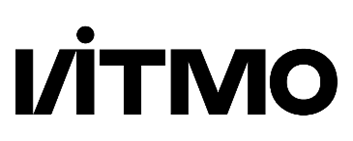
\includegraphics{logo}
\end{figure}
\vspace{-\baselineskip}


\begin{center}
	Федеральное государственное автономное образовательное \\
	учреждение высшего образования\\
	«Национальный исследовательский университет ИТМО»
\end{center}\par

\begin{center}
	\vspace{12pt}
	\Faculty
\end{center}\par

\vspace{\fill}
\begin{center}
	Лабораторная работа \LabNumber \\
	По дисципление: \LabSubject \\
	Тема: <<\LabName>> \\
	Вариант \Variant
\end{center}\par

\vspace{\fill}
\vbox{
	\hfill
	\vbox{
		\hbox{\textbf{Выполнил:} \StudentName}
		\hbox{\textbf{Группа:} \StudentGroup \\}
		\hbox{\textbf{Преподаватель:} \TeacherPosition \TeacherName}
	}
} 


\vspace{\fill}
\begin{center}
	Санкт-Петербург, \the\year{}
\end{center}\par

\newpage

	
	\tableofcontents
	\newpage
	
	\section*{Задание}
	\addcontentsline{toc}{section}{Задание}
	\begin{enumerate}
	\item Создать приведенное в варианте дерево каталогов и файлов с содержимым. В качестве корня дерева использовать каталог lab0 своего домашнего каталога. Для создания и навигации по дереву использовать команды: mkdir, echo, cat, touch, ls, pwd, cd, more, cp, rm, rmdir, mv.
	\begin{figure}[h]
		\centering
		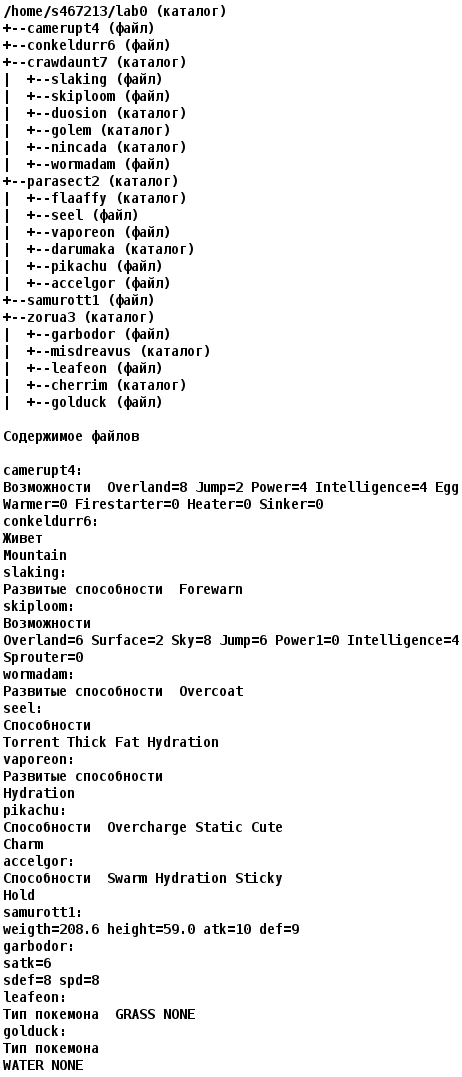
\includegraphics[scale=0.5]{task}
	\end{figure}
	
	\item Установить согласно заданию права на файлы и каталоги при помощи команды chmod, используя различные способы указания прав.
	\begin{itemize}
		\item camerupt4: владелец должен не иметь никаких прав; группа-владелец должна не иметь никаких прав; остальные пользователи должны читать файл
		 \item conkeldurr6: владелец должен читать и записывать файл; группа-владелец должна записывать файл; остальные пользователи должны записывать файл
		 \item crawdaunt7: -wxrwxr-x
		 \item slaking: владелец должен не иметь никаких прав; группа-владелец должна читать и записывать файл; остальные пользователи должны записывать файл
		 \item skiploom: владелец должен не иметь никаких прав; группа-владелец должна читать файл; остальные пользователи должны читать и записывать файл
		 \item duosion: права 555
		 \item golem: права 337
		 \item nincada: права 555
		 \item wormadam: ------rw-
		 \item parasect2: -wx-wxr-x
		 \item flaaffy: rwxr-x-w-
		 \item seel: владелец должен читать и записывать файл; группа-владелец должна читать файл; остальные пользователи должны не иметь никаких прав
		 \item vaporeon: владелец должен читать файл; группа-владелец должна читать файл; остальные пользователи должны не иметь никаких прав
		 \item darumaka: владелец должен читать, записывать директорию и переходить в нее; группа-владелец должна читать директорию и переходить в нее; остальные пользователи должны записывать директорию
		 \item pikachu: владелец должен не иметь никаких прав; группа-владелец должна читать файл; остальные пользователи должны читать и записывать файл
		 \item accelgor: права 044
		 \item samurott1: r--------
		 \item zorua3: r-x--x-wx
		 \item garbodor: владелец должен читать и записывать файл; группа-владелец должна не иметь никаких прав; остальные пользователи должны не иметь никаких прав
		 \item misdreavus: владелец должен читать директорию и переходить в нее; группа-владелец должна только переходить в директорию; остальные пользователи должны записывать директорию и переходить в нее
		 \item leafeon: r-----r--
		 \item cherrim: владелец должен читать директорию и переходить в нее; группа-владелец должна читать, записывать директорию и переходить в нее; остальные пользователи должны читать, записывать директорию и переходить в нее
		 \item golduck: права 640
	\end{itemize}
	
	\item Скопировать часть дерева и создать ссылки внутри дерева согласно заданию при помощи команд cp и ln, а также комманды cat и перенаправления ввода-вывода.
	\begin{itemize}
		\item скопировать рекурсивно директорию parasect2 в директорию lab0/crawdaunt7/nincada
		\item скопировать файл camerupt4 в директорию lab0/crawdaunt7/duosion
		\item cоздать жесткую ссылку для файла conkeldurr6 с именем lab0/crawdaunt7/slakingconkeldurr
		\item создать символическую ссылку c именем Copy\_5 на директорию zorua3 в каталоге lab0
		\item объеденить содержимое файлов lab0/zorua3/golduck, lab0/parasect2/accelgor, в новый файл lab0/camerupt4\_76
		\item скопировать содержимое файла conkeldurr6 в новый файл lab0/parasect2/accelgorconkeldurr
		\item cоздать символическую ссылку для файла camerupt4 с именем lab0/crawdaunt7/slakingcamerupt
	\end{itemize}
	
	\item Используя команды cat, wc, ls, head, tail, echo, sort, grep выполнить в соответствии с вариантом задания поиск и фильтрацию файлов, каталогов и содержащихся в них данных.
	\begin{itemize}
		\item Рекурсивно подсчитать количество символов содержимого файлов из директории lab0, имя которых начинается на 'c', результат записать в файл в директории /tmp, подавить вывод ошибок доступа
		\item Вывести четыре первых элемента рекурсивного списка имен и атрибутов файлов в директории lab0, содержащих строку "da", список отсортировать по убыванию даты модификации файла, подавить вывод ошибок доступа
		\item Рекурсивно вывести содержимое файлов из директории lab0, имя которых заканчивается на 'r', строки отсортировать по имени a->z, ошибки доступа перенаправить в файл в директории /tmp
		\item Вывести содержимое файлов: wormadam, seel, vaporeon, pikachu, accelgor, garbodor, leafeon, исключить строки, заканчивающиеся на 'n', регистр символов игнорировать, добавить вывод ошибок доступа в стандартный поток вывода
		\item Подсчитать количество символов содержимого файлов в директории crawdaunt7, результат записать в файл в директории /tmp, добавить вывод ошибок доступа в стандартный поток вывода
		\item Вывести два первых элемента рекурсивного списка имен и атрибутов файлов в директории lab0, содержащих строку "ldu", список отсортировать по возрастанию даты изменения записи о файле, ошибки доступа перенаправить в файл в директории /tmp
	\end{itemize}
	
	\item Выполнить удаление файлов и каталогов при помощи команд rm и rmdir согласно варианту задания.
	\begin{itemize}
		\item Удалить файл conkeldurr6
		\item Удалить файл lab0/crawdaunt7/wormadam
		\item удалить символические ссылки lab0/crawdaunt7/slakingcameru*
		\item удалить жесткие ссылки lab0/crawdaunt7/slakingconkeldu*
		\item Удалить директорию zorua3
		\item Удалить директорию lab0/parasect2/flaaffy
	\end{itemize}
\end{enumerate}
	
	\section*{Процесс выполнения}
	\addcontentsline{toc}{section}{Процесс выполнени}
	
	\subsection*{Задание 1}
	\addcontentsline{toc}{subsection}{Задание 1}
	\begin{minted}[breaklines]{bash}
#!/usr/bin/bash

# Create root dir
mkdir lab0 && cd lab0

# Create dirs
mkdir crawdaunt7
mkdir crawdaunt7/duosion
mkdir crawdaunt7/golem
mkdir crawdaunt7/nincada

mkdir parasect2
mkdir parasect2/flaaffy
mkdir parasect2/darumaka

mkdir zorua3
mkdir zorua3/misdreavus
mkdir zorua3/cherrim

# Create files
echo "Возможности Overland=8 Jump=2 Power=4 Intelligence=4 Egg" "Warmer 0 Firestarter=0 Heater=0 Sinker=0" > camerupt4
echo "Живет" "Mountain" > conkeldurr6
echo "Развитые способности Forewarn" > crawdaunt7/slaking
echo "Возможности" "Overland=6 Surface=2 Sky=8 Jump=6 Power1=0 Intelligence=4" "Sprouter=0"> crawdaunt7/skiploom
echo "Развитые способности Overcoat" > crawdaunt7/wormadam
echo "Способности" "Torrent Thick Fat Hydration" > parasect2/seel
echo "Развитые способности" "Hydration" > parasect2/vaporeon
echo "Способности Overcharge Static Cute" "Charm"  > parasect2/pikachu
echo "Способности Swarm Hydration Sticky" "Hold" > parasect2/accelgor
echo "weight=208.6 height=59.0 atk=10 def=9" > samurottl
echo "satk=6" "sdef=8 spd=8" > zorua3/garbodor
echo "Тип покемона GRASS NONE" > zorua3/leafeon
echo "Типо покемона" "WATER NONE" > zorua3/golduck
\end{minted}


	
	\subsection*{Задание 2}
	\addcontentsline{toc}{subsection}{Задание 2}
	\begin{minted}[breaklines]{bash}
#!/usr/bin/bash

cd lab0

chmod 004 camerupt4
chmod 622 conkeldurr6

chmod 375 crawdaunt7/

chmod u=,g=rw,o=w crawdaunt7/slaking
chmod u=,g=r,o=rw crawdaunt7/skiploom
chmod 555 crawdaunt7/duosion/
chmod 337 crawdaunt7/golem
chmod 555 crawdaunt7/nincada
chmod u=,g=,o=rw crawdaunt7/wormadam

chmod 335 parasect2/
chmod 752 parasect2/flaaffy/
chmod 640 parasect2/seel
chmod 440 parasect2/vaporeon
chmod 752 parasect2/darumaka/
chmod 046 parasect2/pikachu
chmod 044 parasect2/accelgor

chmod 400 samurottl
chmod 513 zorua3/

chmod u=rw,g=,o= zorua3/garbodor
chmod u=rx,g=x,o=wx zorua3/misdreavus/
chmod u=r,g=,o=r zorua3/leafeon
chmod u=rx,g=rwx,o=rwx zorua3/cherrim/
chmod 640 zorua3/golduck
\end{minted}


	
	\subsection*{Задание 3}
	\addcontentsline{toc}{subsection}{Задание 3}
	\subsubsection*{Cкопировать рекурсивно директорию parasect2 в директорию lab0/crawdaunt7/nincada}
Смена прав: 
\begin{minted}{bash}
chmod u+r parasect2/
chmod u+r parasect2/accelgor
chmod u+r parasect2/pikachu
chmod u+w crawdaunt7/nincada/
\end{minted}

Команда: \mint{bash}|cp -r parasect2 crawdaunt7/nincada|

Результат
\begin{minted}{shell}
[s467213@helios ~/opd/lab0/lab0]$ ls -lp parasect2/ crawdaunt7/nincada/parasect2/
crawdaunt7/nincada/parasect2/:
total 3
-r--r--r--  1 s467213 studs 51  7 окт.  14:32 accelgor
drwxr-x---  2 s467213 studs  2  7 окт.  14:32 darumaka/
drwxr-x---  2 s467213 studs  2  7 окт.  14:32 flaaffy/
-r--r--r--  1 s467213 studs 52  7 окт.  14:32 pikachu
-rw-r-----  1 s467213 studs 51  7 окт.  14:32 seel
-r--r-----  1 s467213 studs 50  7 окт.  14:32 vaporeon

parasect2/:
total 3
-r--r--r--  1 s467213 studs 51  7 окт.  14:32 accelgor
drwxr-x-w-  2 s467213 studs  2  7 окт.  14:32 darumaka/
drwxr-x-w-  2 s467213 studs  2  7 окт.  14:32 flaaffy/
-r--r--rw-  1 s467213 studs 52  7 окт.  14:32 pikachu
-rw-r-----  1 s467213 studs 51  7 окт.  14:32 seel
-r--r-----  1 s467213 studs 50  7 окт.  14:32 vaporeon
\end{minted}

Возвращаем права:
\begin{minted}{bash}
chmod u-r parasect2/
chmod u-r parasect2/accelgor
chmod u-r parasect2/pikachu
chmod u-w crawdaunt7/nincada/
\end{minted}

\subsubsection*{Скопировать файл camerupt4 в директорию lab0/crawdaunt7/duosion}
Смена прав: 
\begin{minted}{bash}
chmod u+r camerupt4
chmod u+w crawdaunt7/duosion
\end{minted}

Команда: \mint{bash}|cp camerupt4 crawdaunt7/duosion|

Результат
\begin{minted}{shell}
[s467213@helios ~/opd/lab0/lab0]$ ls -l crawdaunt7/duosion
total 5
-r-----r--  1 s467213 studs 109  6 окт.  15:21 camerupt4
\end{minted}

Возвращаем права:
\begin{minted}{bash}
chmod u-r camerupt4
chmod u-w crawdaunt7/duosion
\end{minted}


\subsubsection*{Создать жесткую ссылку для файла conkeldurr6 с именем lab0/crawdaunt7/slakingconkeldurr}

Команда: \mint{bash}|ln conkeldurr6 crawdaunt7/slakingconkeldurr|

Результат
\begin{minted}{shell}
[s467213@helios ~/opd/lab0/lab0]$ ls -li conkeldurr6 crawdaunt7/slakingconkeldurr
8471566 -rw--w--w-  2 s467213 studs 20  6 окт.  15:24 conkeldurr6
8471566 -rw--w--w-  2 s467213 studs 20  6 окт.  15:24 crawdaunt7/slakingconkeldurr
\end{minted}

\subsubsection*{Создать символическую ссылку c именем Copy\_5 на директорию zorua3 в каталоге lab0}
Команда: \mint{bash}|ln -s zorua3/ Copy_5|

Результат
\begin{minted}{shell}
[s467213@helios ~/opd/lab0/lab0]$ ls -l Copy_5
lrwxr-xr-x  1 s467213 studs 7  7 окт.  14:16 Copy_5 -> zorua3/
[s467213@helios ~/opd/lab0/lab0]$ file Copy_5
Copy_5: symbolic link to zorua3/
[s467213@helios ~/opd/lab0/lab0]$
\end{minted}

\subsubsection*{Объеденить содержимое файлов lab0/zorua3/golduck, lab0/parasect2/accelgor, в новый файл lab0/camerupt4\_76}

Смена прав: 
\begin{minted}{bash}
chmod u+r parasect2/accelgor
\end{minted}

Команда: \mint{bash}|cat zorua3/golduck parasect2/accelgor > camerupt4_76|

Результат
\begin{minted}{shell}
[s467213@helios ~/opd/lab0/lab0]$ cat zorua3/golduck parasect2/accelgor camerupt4_76
Типо покемона WATER NONE
Способности Swarm Hydration Sticky Hold
Типо покемона WATER NONE
Способности Swarm Hydration Sticky Hold
\end{minted}

Возвращаем права:
\begin{minted}{bash}
chmod u-r parasect2/accelgor
\end{minted}


\subsubsection*{Скопировать содержимое файла conkeldurr6 в новый файл lab0/parasect2/accelgorconkeldurr}
Команда: \mint{bash}|cat conkeldurr6 > parasect2/accelgorconkeldurr|

Результат
\begin{minted}{shell}
[s467213@helios ~/opd/lab0/lab0]$ cat conkeldurr6 parasect2/accelgorconkeldurr
Живет Mountain
Живет Mountain
\end{minted}

\subsubsection*{Создать символическую ссылку для файла camerupt4 с именем lab0/crawdaunt7/slakingcamerupt}
Команда: \mint{bash}|ln -s $PWD/camerupt4 crawdaunt7/slakingcamerupt|

Результат
\begin{minted}{shell}
[s467213@helios ~/opd/lab0/lab0]$ ls -l crawdaunt7/slakingcamerupt
lrwxr-xr-x  1 s467213 studs 43  7 окт.  14:27 crawdaunt7/slakingcamerupt -> /home/studs/s467213/opd/lab0/lab0/camerupt4
[s467213@helios ~/opd/lab0/lab0]$ file crawdaunt7/slakingcamerupt
crawdaunt7/slakingcamerupt: symbolic link to /home/studs/s467213/opd/lab0/lab0/camerupt4
\end{minted}

	
	\subsection*{Древо каталогов после 3-го задания}
	\addcontentsline{toc}{subsection}{Древо каталогов после 3-го задания}
	\begin{minted}[breaklines]{shell}
[s467213@helios ~/opd/lab0]$ ls -Rp lab0/
camerupt4       conkeldurr6     crawdaunt7/     samurottl
camerupt4_76    Copy_5          parasect2/      zorua3/

lab0/crawdaunt7:
ls: lab0/crawdaunt7: Permission denied

lab0/parasect2:
ls: lab0/parasect2: Permission denied

lab0/zorua3:
cherrim/        garbodor        golduck         leafeon         misdreavus/

lab0/zorua3/cherrim:

lab0/zorua3/misdreavus:
\end{minted}


	
	\subsection*{Задание 4}
	\addcontentsline{toc}{subsection}{Задание 4}
	\subsubsection*{Рекурсивно подсчитать количество символов содержимого файлов из директории lab0, имя которых начинается на 'c', результат записать в файл в директории /tmp, подавить вывод ошибок доступа}
\begin{minted}[breaklines]{shell}
[s467213@helios ~/opd/lab0/lab0]$ cat c* */c* */*/c* 2> /dev/null | wc -m > /tmp/131
[s467213@helios ~/opd/lab0/lab0]$ cat /tmp/131
80
\end{minted}


\subsubsection*{Вывести четыре первых элемента рекурсивного списка имен и атрибутов файлов в директории lab0, содержащих строку `da`, список отсортировать по убыванию даты модификации файла, подавить вывод ошибок доступа}
\begin{minted}[breaklines]{shell}
[s467213@helios ~/opd/lab0/lab0]$ ls -Rl 2> /dev/null | grep "^[-|l]" | grep ":[0-6][0-9] \w*da" | sort -rk6 | head -n4
-rw-r--r--  1 s467213 studs   0 17 окт.  13:51 alakyda
-rw-r--r--  1 s467213 studs   0 17 окт.  13:48 dautdat
\end{minted}

\subsubsection*{Рекурсивно вывести содержимое файлов из директории lab0, имя которых заканчивается на 'r', строки отсортировать по имени a->z, ошибки доступа перенаправить в файл в директории /tmp}
\begin{minted}[breaklines]{shell}
[s467213@helios ~/opd/lab0/lab0]$ cat *r */*r */*/*r 2> /tmp/13_3 | sort
allow any
satk=6 sdef=8 spd=8
satk=6 sdef=8 spd=8
\end{minted}

\subsubsection*{Вывести содержимое файлов: wormadam, seel, vaporeon, pikachu, accelgor, garbodor, leafeon, исключить строки, заканчивающиеся на 'n', регистр символов игнорировать, добавить вывод ошибок доступа в стандартный поток вывода}
\begin{minted}[breaklines]{shell}
[s467213@helios ~/opd/lab0/lab0]$ cat crawdaunt7/wormadam parasect2/seel parasect2/vaporeon parasect2/pikachu parasect2/accelgor zorua3/garbodor zorua3/leafeon 2>&1 | grep -v [nN]$
cat: crawdaunt7/wormadam: Permission denied
cat: parasect2/pikachu: Permission denied
cat: parasect2/accelgor: Permission denied
satk=6 sdef=8 spd=8
Тип покемона GRASS NONE
\end{minted}

\subsubsection*{Подсчитать количество символов содержимого файлов в директории crawdaunt7, результат записать в файл в директории /tmp, добавить вывод ошибок доступа в стандартный поток вывода}
\begin{minted}[breaklines]{shell}
[s467213@helios ~/opd/lab0/lab0]$ cat crawdaunt7/* 2>&1 | grep -v "^cat" | wc -m > /tmp/135
[s467213@helios ~/opd/lab0/lab0]$ cat /tmp/135
15
\end{minted}

\subsubsection*{Вывести два первых элемента рекурсивного списка имен и атрибутов файлов в директории lab0, содержащих строку `ldu`, список отсортировать по возрастанию даты изменения записи о файле, ошибки доступа перенаправить в файл в директории /tmp}
\begin{minted}[breaklines]{shell}
[s467213@helios ~/opd/lab0/lab0]$ ls -lR 2> /tmp/136_err | grep "^[-|l]" | grep ":[0-6][0-9] \w*ldu" | sort -k6 | head -n2
-rw--w--w-  2 s467213 studs  20  7 окт.  10:12 conkeldurr6
-rw-r-----  1 s467213 studs 37  7 окт.  10:12 golduck
\end{minted}
	
	\subsection*{Задание 5}
	\addcontentsline{toc}{subsection}{Задание 5}
	Скрипт
\begin{minted}[breaklines]{bash}
#!/usr/bin/bash

cd lab0

# Удалить файл conkeldurr6
rm -v conkeldurr6

# Удалить файл lab0/crawdaunt7/wormadam
rm -fv crawdaunt7/wormadam

# Удалить символические ссылки lab0/crawdaunt7/slakingcameru*
rm -v crawdaunt7/slakingcameru*

# Удалить жесткие ссылки lab0/crawdaunt7/slakingconkeldu*
rm -v crawdaunt7/slakingconkeldu*

# Удалить директорию zorua3
chmod -R u+w zorua3/
rm -rv zorua3/

# Удалить директорию lab0/parasect2/flaaffy
rmdir parasect2/flaaffy
\end{minted}

Результат
\begin{minted}[breaklines]{shell}
[s467213@helios ~/opd/lab0]$ ./task_5.sh
conkeldurr6
crawdaunt7/wormadam
crawdaunt7/slakingcamerupt
crawdaunt7/slakingconkeldurr
zorua3/leafeon
zorua3/golduck
zorua3/garbodor
zorua3/misdreavus
zorua3/cherrim
zorua3/
parasect2/flaaffy
[s467213@helios ~/opd/lab0]$ ls -lR lab0/
total 23
-------r--  1 s467213 studs 109  6 окт.  16:18 camerupt4
-rw-r--r--  1 s467213 studs  88  6 окт.  16:18 camerupt4_76
lrwxr-xr-x  1 s467213 studs   7  6 окт.  16:18 Copy_5 -> zorua3/
drwxrwxr-x  5 s467213 studs   7  6 окт.  16:18 crawdaunt7
d-wx-wxr-x  3 s467213 studs   8  6 окт.  16:18 parasect2
-r--------  1 s467213 studs  38  6 окт.  16:18 samurottl

lab0/crawdaunt7:
total 3
dr-xr-xr-x  2 s467213 studs  3  6 окт.  16:18 duosion
d-wx-wxrwx  2 s467213 studs  2  6 окт.  16:18 golem
drwxr-xr-x  3 s467213 studs  3  6 окт.  16:18 nincada
----r--rw-  1 s467213 studs 92  6 окт.  16:18 skiploom
----rw--w-  1 s467213 studs 49  6 окт.  16:18 slaking

lab0/crawdaunt7/duosion:
total 5
-r-----r--  1 s467213 studs 109  6 окт.  16:18 camerupt4

lab0/crawdaunt7/golem:
total 0
ls: lab0/crawdaunt7/golem: Permission denied

lab0/crawdaunt7/nincada:
total 9
drwx--xr-x  4 s467213 studs 8  6 окт.  16:18 parasect2

lab0/crawdaunt7/nincada/parasect2:
total 3
-r--r--r--  1 s467213 studs 51  6 окт.  16:18 accelgor
drwxr-x---  2 s467213 studs  2  6 окт.  16:18 darumaka
drwxr-x---  2 s467213 studs  2  6 окт.  16:18 flaaffy
-r--r--r--  1 s467213 studs 52  6 окт.  16:18 pikachu
-rw-r-----  1 s467213 studs 51  6 окт.  16:18 seel
-r--r-----  1 s467213 studs 50  6 окт.  16:18 vaporeon

lab0/crawdaunt7/nincada/parasect2/darumaka:
total 0

lab0/crawdaunt7/nincada/parasect2/flaaffy:
total 0

lab0/parasect2:
total 0
ls: lab0/parasect2: Permission denied
\end{minted}
	
	\section*{Вывод}
	\addcontentsline{toc}{section}{Вывод}
	В процессе выполнения работы я:
\begin{itemize}
	\item познакомился с основами ООП в Java
	\item научился подключать сторонние .jar  библиотеки
	\item познакомился с системой сборки Gradle и научился создавать  fatJar с её помощью
\end{itemize}
	
\end{document}